\documentclass[bwprint]{gmcmthesis}
\usepackage{amsmath}
\usepackage{pdfpages}
\usepackage{graphicx}
\usepackage{subcaption}
\numberwithin{figure}{section}

\title{Computer Vision Homework 1 Report}

\author{涂宇清 522030910152}
\date{}

\begin{document}
\setlength{\parskip}{10pt}
\baselineskip=1.5\baselineskip
% \linespread{0.1}
\maketitle

\section{Written Assignment}
\subsection{Problem 1}
\begin{enumerate}[label=\alph*.]
    \item Assume that the origin is the pinhole and the circular disk's center is in $(x_0, y_0, z_0)$ and the radius is $r$. The equation of the circular disk is:
    \begin{equation}
        (x - x_0)^2 + (y - y_0)^2 = r^2, \quad z = z_0
    \end{equation}
    Assume the effective focal length is $f$. The projection of the circular disk on the image plane is:
    \begin{equation}
        \frac{x_p}{f} = \frac{x}{z_0}, \quad \frac{y_p}{f} = \frac{y}{z_0}
    \end{equation}
    Then the projection of the circular disk on the image plane is:
    \begin{equation}
        \left(x_p - \frac{x_0f}{z_0}\right)^2 + \left(y_p - \frac{y_0f}{z_0}\right)^2 = \left(\frac{rf}{z_0}\right)^2
    \end{equation}
    So the projection of the circular disk on the image plane is a circle with center $(\frac{x_0f}{z_0}, \frac{y_0f}{z_0})$ and radius $\frac{rf}{z_0}$.

    \item \begin{itemize}
        \item For $A=C=D=0$ and $B=1$, assume three line directions are $(1, 0, 1)$, $(0, 0, 1)$ and $(-1, 0, 1)$. According to the vanishing point formula:
        \begin{equation}
            \left(x_{vp}, y_{vp}\right) = \left(f\frac{l_x}{l_z}, f\frac{l_y}{l_z}\right)
        \end{equation}
        The vanishing point of the three line directions are $(f, 0)$, $(0, 0)$ and $(-f, 0)$.
        \item For $B=C=D=0$ and $A=1$, assume three line are $(0, 1, 1)$, $(0, 0, 1)$ and $(0, -1, 1)$. The vanishing point of the three lines are $(0, f)$, $(0, 0)$ and $(0, -f)$.
    \end{itemize}

    \item For the general case, the plane equation is $Ax + By + Cz + D = 0$. We assume that there are anys two different points $(x_1, y_1, z_1)$ and $(x_2, y_2, z_2)$ on the plane. Then we have:
    \begin{equation}
        \begin{aligned}
            Ax_1 + By_1 + Cz_1 + D &= 0 \\
            Ax_2 + By_2 + Cz_2 + D &= 0
        \end{aligned}
    \end{equation}
    And we know that any line direction can be presented as $(l_x, l_y, l_z) = (x_1 - x_2, y_2 - y_1, z_1 - z_2)$. So we have:
    \begin{equation}
        \begin{aligned}
            A(x_1 - x_2) + B(y_2 - y_1) + C(z_1 - z_2) &= 0 \\
            Al_x + Bl_y + Cl_z &= 0 \\
            Ax_{vp} + By_{vp} + Cf &= 0
        \end{aligned}
    \end{equation}
    So the vanishing point satisfies the equation $Ax + By + Cf = 0$.
\end{enumerate}

\section{Programming Assignment}
\subsection{Problem 1}
\begin{enumerate}[label=\alph*.]
    \item Choose 128 as the threshold. The result is shown in Figure \ref{fig:subfigure2} and \ref{fig:subfigure6}.
    \item Each connected region is labeled with a different color. The result is shown in Figure \ref{fig:subfigure3} and \ref{fig:subfigure7}.
    \item Use the formulas that we have learned in the class. The result is shown in Figure \ref{fig:subfigure4} and \ref{fig:subfigure8}.
    \begin{figure}[h]
        \centering
        \begin{subfigure}[b]{0.3\textwidth}
            \centering
            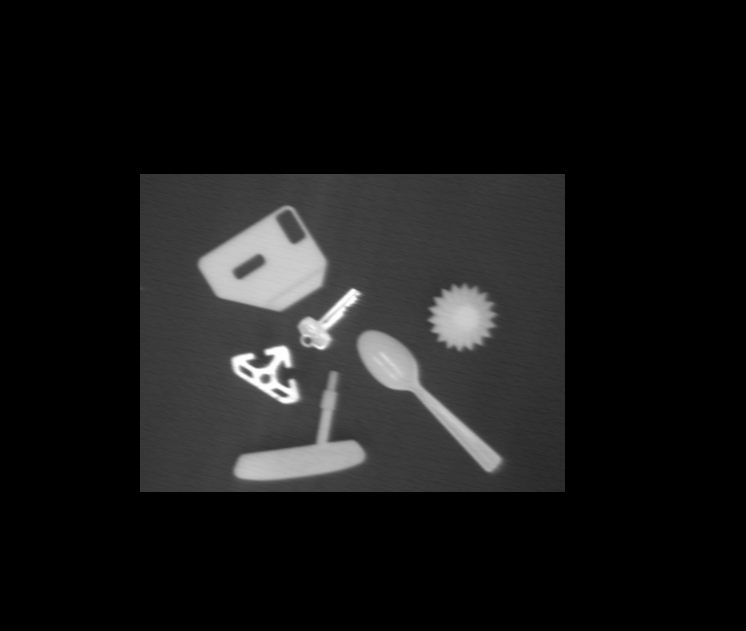
\includegraphics[width=\textwidth]{../output/many_objects_1_gray.png}
            \caption{many\_objects\_1\_gray}
            \label{fig:subfigure1}
        \end{subfigure}
        \hfill
        \begin{subfigure}[b]{0.3\textwidth}
            \centering
            
\includegraphics[width=\textwidth]{../output/many_objects_1_binary.png}
            \caption{many\_objects\_1\_binary}
            \label{fig:subfigure2}
        \end{subfigure}
        \hfill
        \begin{subfigure}[b]{0.3\textwidth}
            \centering
            
\includegraphics[width=\textwidth]{../output/many_objects_1_labeled.png}
            \caption{many\_objects\_1\_labeled}
            \label{fig:subfigure3}
        \end{subfigure}
        \newline
        \begin{subfigure}[b]{\textwidth}
            \centering
            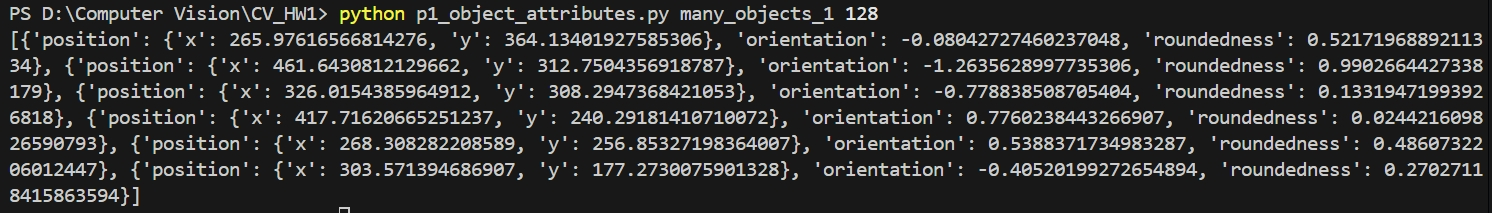
\includegraphics[width=\textwidth]{../output/many_objects_1_attribute.png}
            \caption{many\_objects\_1\_attribute}
            \label{fig:subfigure4}
        \end{subfigure}
        \newline

        \centering
        \begin{subfigure}[b]{0.3\textwidth}
            \centering
            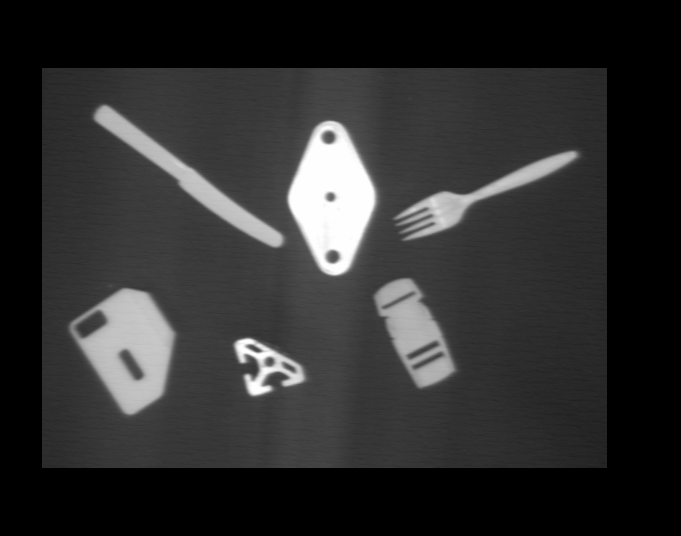
\includegraphics[width=\textwidth]{../output/many_objects_2_gray.png}
            \caption{many\_objects\_2\_gray}
            \label{fig:subfigure5}
        \end{subfigure}
        \hfill
        \begin{subfigure}[b]{0.3\textwidth}
            \centering
            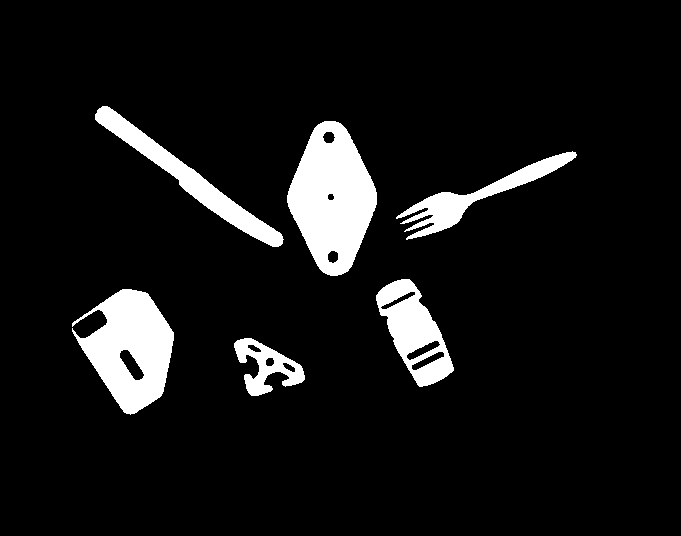
\includegraphics[width=\textwidth]{../output/many_objects_2_binary.png}
            \caption{many\_objects\_2\_binary}
            \label{fig:subfigure6}
        \end{subfigure}
        \hfill
        \begin{subfigure}[b]{0.3\textwidth}
            \centering
            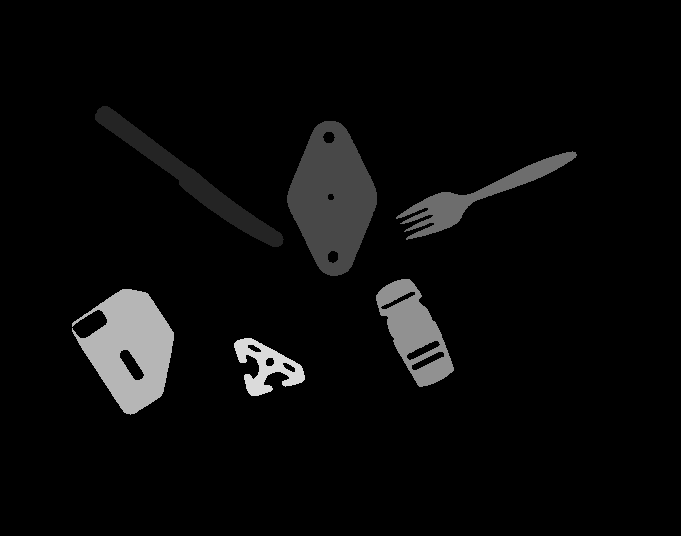
\includegraphics[width=\textwidth]{../output/many_objects_2_labeled.png}
            \caption{many\_objects\_2\_labeled}
            \label{fig:subfigure7}
        \end{subfigure}
        \newline
        \begin{subfigure}[b]{\textwidth}
            \centering
            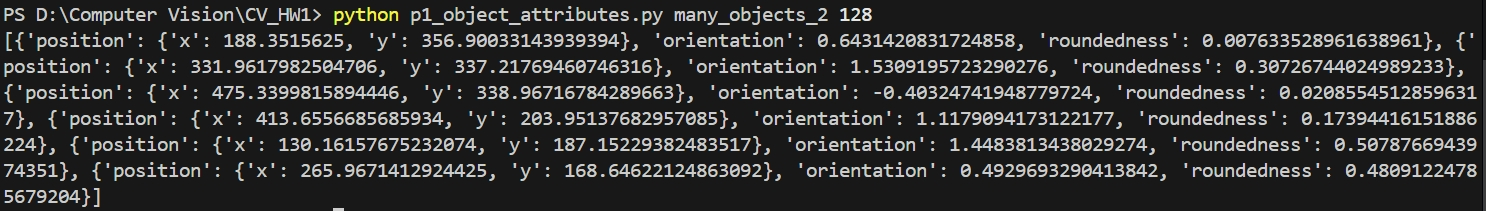
\includegraphics[width=\textwidth]{../output/many_objects_2_attribute.png}
            \caption{many\_objects\_2\_attribute}
            \label{fig:subfigure8}
        \end{subfigure}
    \caption{Results of Problem 1}
    \end{figure}
\end{enumerate}

\subsection{Problem 2}
\begin{enumerate}[label=\alph*.]
    \item Choose $[[-1, 0, 1], [-2, 0, 2], [-1, 0, 1]]$ and $[[1, 2, 1], [0, 0, 0], [-1, -2, -1]]$ as kernels of Sobel edge detector. The result is shown in Figure \ref{fig:subfigure9}.
    \item Choose 128 as the edge threshold and $[20, 21, \cdots, 30, 40]$ as radius values. The result of get edges is shown in Figure \ref{fig:subfigure10}.
    \item Choose 80 as the Hough vote threshold. Final circle edges are shown in Figure \ref{fig:subfigure11} and the attributes of the circle edges are shown in Figure \ref{fig:subfigure12}.
\end{enumerate}

\begin{figure}[h]
    \begin{subfigure}[b]{0.3\textwidth}
        \centering
        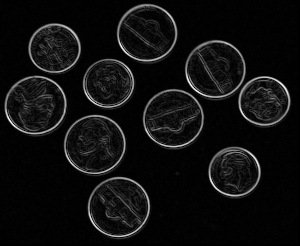
\includegraphics[width=\textwidth]{../output/coins_edges_sobel.png}
        \caption{coins\_edges\_sobel}
        \label{fig:subfigure9}
    \end{subfigure}
    \hfill
    \begin{subfigure}[b]{0.3\textwidth}
        \centering
        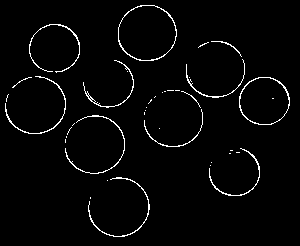
\includegraphics[width=\textwidth]{../output/coins_edges.png}
        \caption{coins\_edges}
        \label{fig:subfigure10}
    \end{subfigure}
    \hfill
    \begin{subfigure}[b]{0.3\textwidth}
        \centering
        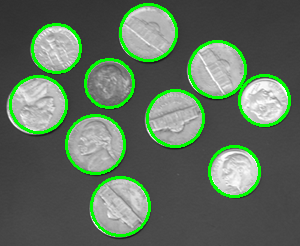
\includegraphics[width=\textwidth]{../output/coins_circles.png}
        \caption{coins\_circles}
        \label{fig:subfigure11}
    \end{subfigure}
    \newline
    \begin{subfigure}[b]{\textwidth}
        \centering
        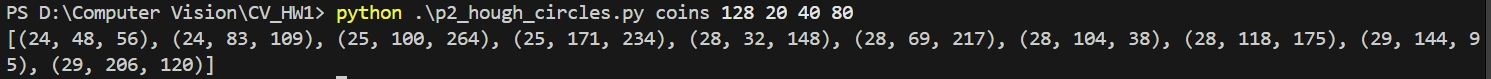
\includegraphics[width=\textwidth]{../output/coins_attribute.png}
        \caption{coins\_attribute}
        \label{fig:subfigure12}
    \end{subfigure}
    \caption{Results of Problem 2}
\end{figure}

\end{document} 
